\documentclass[class=report, crop=false, 12pt,a4paper]{standalone}
\usepackage{float}
\usepackage{graphicx}
\usepackage{siunitx}
\usepackage{mathtools}
\usepackage{amsmath}
\usepackage{amssymb}
\usepackage{commath}
\usepackage[a4paper,width=150mm,top=25mm,bottom=25mm]{geometry}
\begin{document}
\section{The s-Plane - Poles and Zeroes}
\subsection{Example: Servo as a second order system}
\begin{figure}[H]
  \centering
  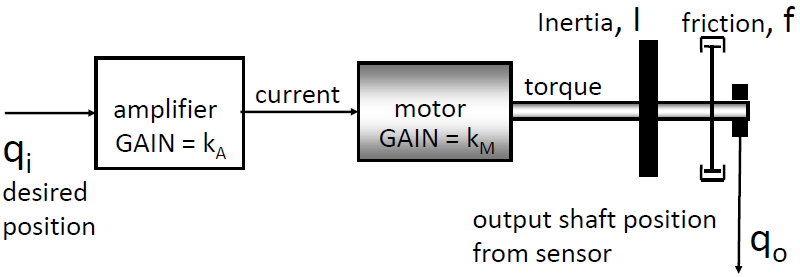
\includegraphics[width = 0.6\textwidth]{../img/diagram87.png}
  \caption{}
\end{figure}
We saw last week that a DC motor servo with position control has a transfer function of a second order system.
\begin{figure}[H]
  \centering
  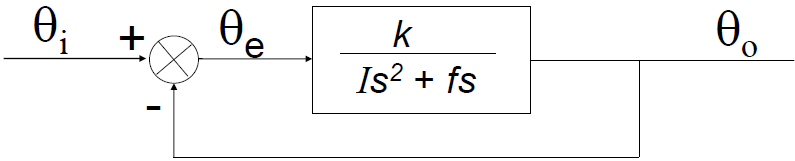
\includegraphics[width = 0.6\textwidth]{../img/diagram88.png}
  \caption{}
\end{figure}
\begin{align}
  F(s) = \frac{G(s)}{1+G(s)} = \frac{\frac{K}{I}}{s^2 + \frac{f}{I}s + \frac{K}{I}}
\end{align}
Where, $\omega_n = \sqrt{\frac{k}{I}}$ (with increasing $k$, $\omega_n$ increases) and $\zeta = \frac{f}{2\sqrt{kI}}$ (with increasing $k$, $\zeta$ decreases).
\begin{figure}[H]
  \centering
  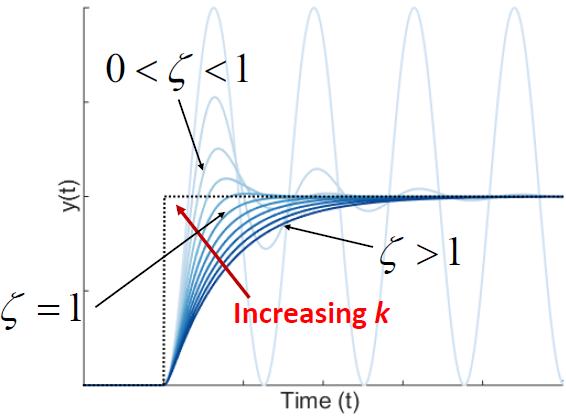
\includegraphics[width = 0.6\textwidth]{../img/diagram89.png}
  \caption{}
\end{figure}
The overdamped ($\zeta > 1$) and critically damped ($\zeta = 1$) responses are seldom desirable for control systems due to their long settling time. $\zeta = 0.7$ gives a fast response without excessive overshoot or oscillations.
\subsection{Transfer functions}
As we have seen, transfer functions allow for important characteristics of the system response to be determined, without having to solve complete differential equations. Generally, transfer functions can be derived from the differential equations thusly: 
\begin{multline}
  a_n \frac{\dif^n y}{\dif t^n} + a_{n-1}\frac{\dif^{n-1} y}{\dif t^{n-1}} + ... + a_2 \frac{\dif^2 y}{\dif t^2} + a_1 \frac{\dif y}{\dif t} + a_0 y =\\ b_0 x + b_1 \frac{\dif x}{\dif t} + b_2 \frac{\dif^2 x}{\dif t^2} + ... + b_{m-1}\frac{\dif^{m-1} x}{\dif t^{m-1}} + b_m \frac{\dif^{m} x}{\dif t^m} \label{TFEq1}
\end{multline}
(Solving equation (\ref{TFEq1}) is hard!). Where $a$ are the output coefficients and $b$ are the input coefficients, combined these \textbf{entirely} characterise the system. The Laplace domain transfer function is then given by:
\begin{align}
  G(s) = \frac{b_m s^m + b_{m-1} s^{m-1} + ... + b_1 s + b_0}{a_n s^n + a_{n-1} s^{n-1} + ... + a_1 s + a_0}
\end{align}
\subsection{System poles and zeroes}
As defined, the transfer function is a rational function in the complex variable $s=\sigma + j\omega$, that is:
\begin{equation}
  G(s) = \frac{b_m s^m + b_{m-1} s^{m-1} + ... + b_1 s + b_0}{a_n s^n + a_{n-1} s^{n-1} + ... + a_1 s + a_0}
\end{equation}
It is often convenient to factor the polynomials in the numerator and denominator; and to write the transfer function in terms of those factors:
\begin{equation}
  G(s) = \frac{N(s)}{D(s)} = K\frac{(s-z_1)(s-z_2)...(s-z_{m-1})(s-z_m)}{(s-p_1)(s-p_2)...(s-p_{n-1})(s-p_n)}
\end{equation}
where the numerator and denominator polynomials, $N(s)$ and $D(s)$, have real coefficients defined by the system's differential equation. Poles and zeroes are found by:
\begin{equation}
  N(s) = 0 \textrm{ and } D(s) = 0
\end{equation}
All of the coefficients of polynomials $N(s)$ and $D(s)$ are real, therefore the poles and zeroes must be either purely real, or appear in complex conjugate pairs.
\begin{quotation}
  The poles and zeros are properties of the transfer function, and therefore of the differential equation describing the input-output system dynamics. Together with the gain constant, they completely characterise the differential equation and provide a complete description of the system.
\end{quotation}
\subsection{Transfer functions in the s-plane}
A system is characterised by its poles and zeroes as they allow the reconstruction of the input/output differential equation. It is possible to get a sense of the system dynamics from plotting the poles and zeroes graphically on the s-plane. A pole is commonly represented by a cross ($\times$) and a zero by a circle ($\circ$). Recall that, as $s$ is a complex number, we can plot the value on a plane, with a real and imaginary axis. 
\begin{equation}
  s = \sigma + j\omega
\end{equation}
By plotting the locations of the poles and zeroes on this plane, we can obtain a considerable amount of information about the response of the system without having to take the inverse Laplace transform. Each pole corresponds to a component of the time domain response, so from the plot it is possible to determine:
\begin{itemize}
  \item What components exist
  \item Their relative important (and possible simplifications)
  \item How they change with gain
\end{itemize}
\subsubsection{Real poles - exponentials}
First lets look at the real component only:
\begin{gather}
  s = \sigma\\
  e^s \rightarrow e^{-\sigma}
\end{gather}
Corresponding to $Ce^{-\sigma t}$
\begin{figure}[H]
  \centering
  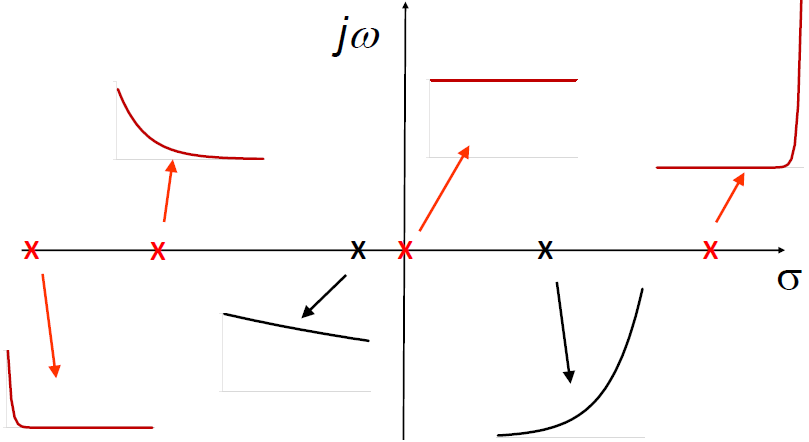
\includegraphics[width = 0.6\textwidth]{../img/diagram90.png}
  \caption{}
\end{figure}
Poles located on the real axis have an exponential component only, with the pole location determining the rate of decay. Poles close to origin decay slowly, where poles far away decay rapidly. Poles located in the right hand side exponentially \textbf{increase}, whereas poles on the left hand side \textbf{decrease}. A pole on the origin is a flat 'DC' response.
\subsubsection{Imaginary poles - sinusoids}
First lets looks at the imaginary component only:
\begin{gather}
  s = \pm j\omega\\
  e^s \rightarrow e^{\pm j\omega}
\end{gather}
Which, from Euler's formula gives a sinusoidal response:
\begin{equation}
  e^{jx} = \cos{x} + j\sin{x}
\end{equation}
Poles located on the imaginary axis are in conjugate pairs.
\begin{figure}[H]
  \centering
  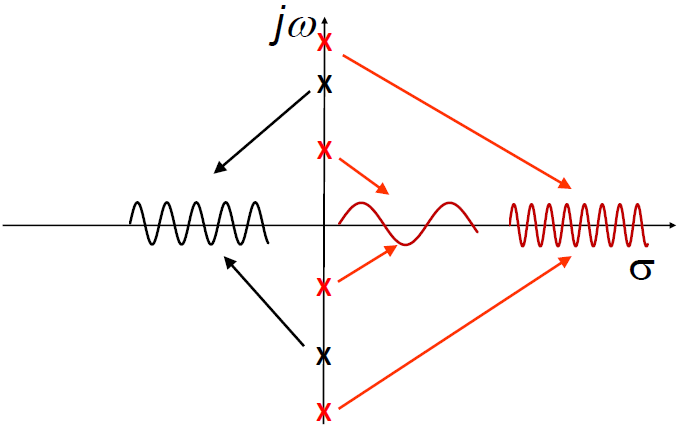
\includegraphics[width = 0.6\textwidth]{../img/diagram91.png}
  \caption{}
\end{figure}
The imaginary poles generate an oscillatory component with a constant amplitude. Poles closer to the origin have a low frequency, which increases the further poles are from the origin.
\subsubsection{Complex poles}
Commonly, the poles are a combination of the two components.
\begin{figure}[H]
  \centering
  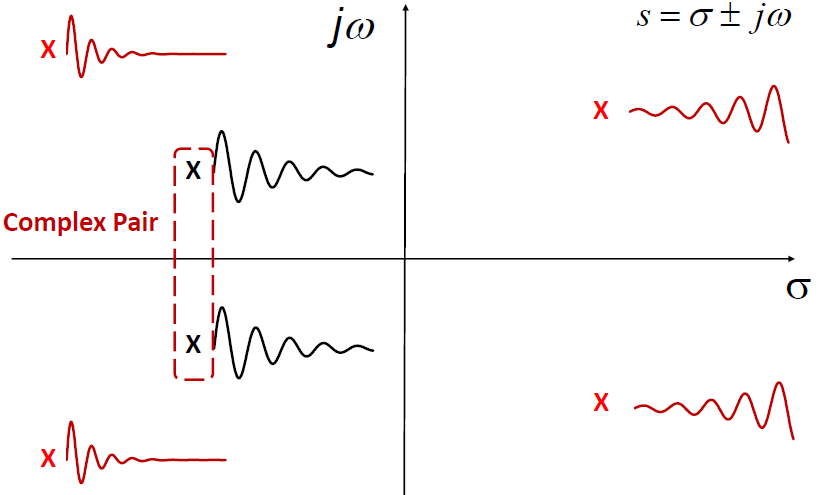
\includegraphics[width = 0.6\textwidth]{../img/diagram92.png}
  \caption{}
\end{figure}
A complex conjugate pair of complex poles generates an exponentially decaying sinusoid in the form: 
\begin{equation}
  Ae^{-\sigma t}\sin{\left(\omega t + \phi\right)}
\end{equation}
$A$ and $\phi$ are determined by the initial conditions, with $\omega$ specifying oscillations and $\sigma$ the rate of decay. Poles located in the left hand side decay to zero, whereas poles in the right hand side increase to infinity, thus making the system \textbf{unstable}.
\subsection{Summary}
The impulse response of each pole in the transfer function depends upon its location in the s-plane:
\begin{figure}[H]
  \centering
  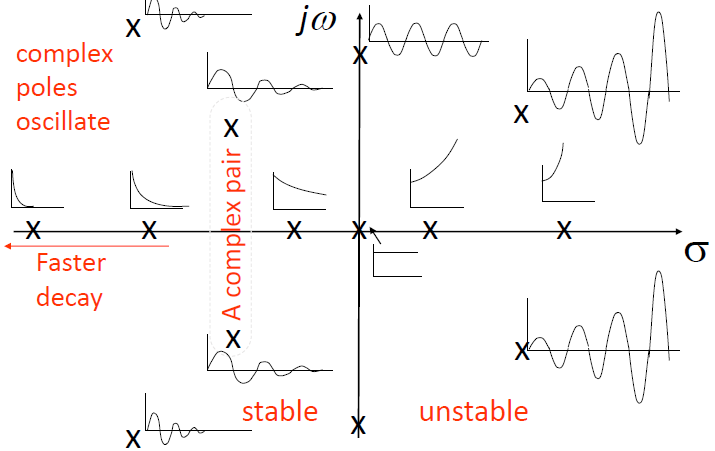
\includegraphics[width = 0.6\textwidth]{../img/diagram93.png}
  \caption{}
\end{figure}
\section{Effects of the damping ratio on poles}
\subsection{Transfer functions of second order systems}
As we have seen, the roots of the transfer function of a second order system depends upon the damping coefficient:
\begin{align}
  G(s) = \frac{\omega_n^2}{s^2 + 2 \zeta \omega_n + \omega_n^2}
\end{align}
We can plot the poles of the characteristic equation as with any other transfer function:
\begin{align}
  s = -\zeta \omega_n \pm \omega_n \sqrt{\zeta^2 - 1}
\end{align}
\subsubsection{Overdamped}
Both roots are real, and thus are on the real axis:
\begin{align}
  s_1 &= -\zeta \omega_n + \omega_n \sqrt{\zeta^2 - 1}\\
  s_2 &= -\zeta \omega_n - \omega_n \sqrt{\zeta^2 - 1}
\end{align}
No oscillations in the step response.
\begin{figure}[H]
  \centerline{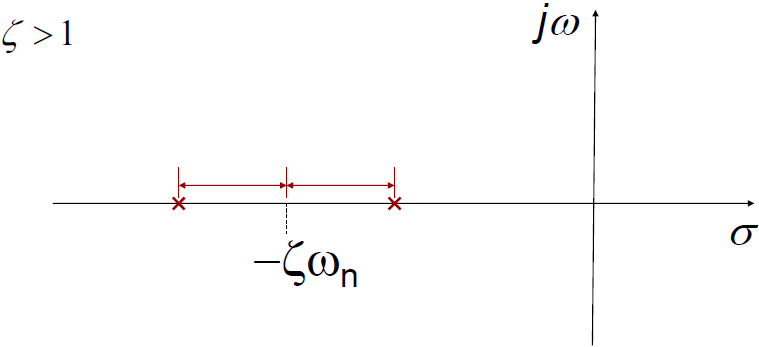
\includegraphics[width = 0.6\textwidth]{../img/diagram94.png}}
  \caption{}
\end{figure}
The \textbf{right} most pole with smallest value of $\sigma$ dominates the response (this was the $\beta$ term from Lecture 5). Further increasing damping ratio, widens the gap between the two poles and shifts them both further away from the origin. Conversely, decreasing the damping ratio brings the two poles closer together, until we reach the special case where $\zeta = 1$.
\subsubsection{Crtically damped}
\begin{figure}[H]
  \centerline{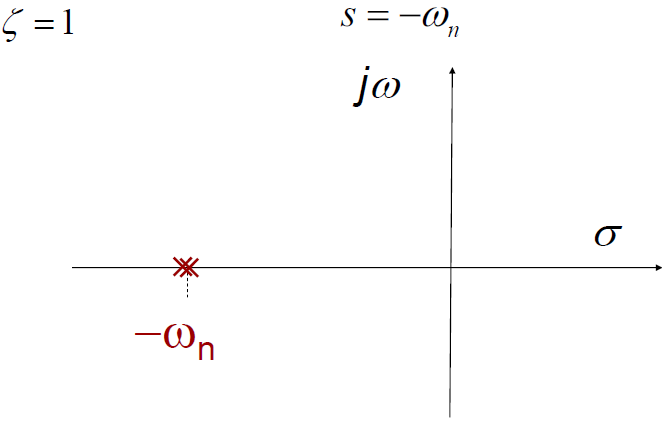
\includegraphics[width = 0.6\textwidth]{../img/diagram95.png}}
  \caption{}
\end{figure}
The roots of the equations coincide, and the system is a product of two equal first order lags.
\subsubsection{Underdamped}
\begin{figure}[H]
  \centerline{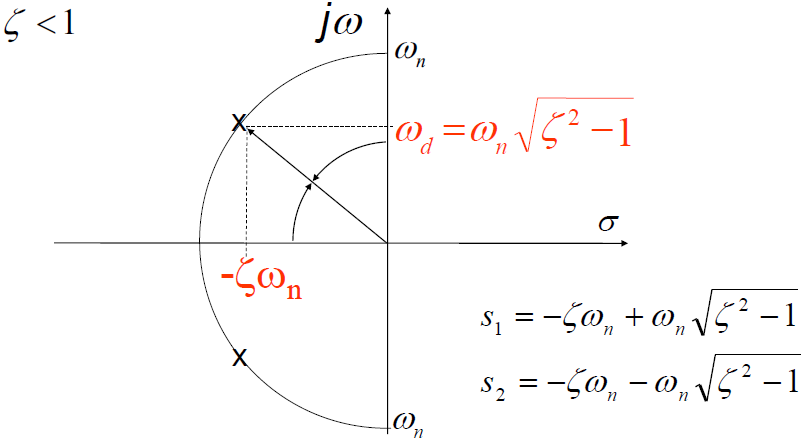
\includegraphics[width = 0.6\textwidth]{../img/diagram96.png}}
  \caption{}
\end{figure}
Both roots complex, and form conjugate pair. System is a product of exponential function and oscillatory component. 
\subsection{Example: Servomechanism in the s-plane}
\begin{align}
  F(s) &= \frac{\frac{k}{I}}{s^2 + \frac{f}{I}s + \frac{k}{I}}\\
  \zeta &= \frac{f}{2\sqrt{kI}}\\
  \omega_n &= \sqrt{\frac{k}{I}}
\end{align}
Considering the second order model for a servo, the roots of the characteristic equation in terms of the parameters $I$, $f$ and $k$ are: 
\begin{equation}
  s = - \frac{f}{2I} \pm \frac{1}{2I} \sqrt{f^2 - 4kI}
\end{equation}
Thus if $f^2 < 4kI$ roots are complex and there is an oscillatory response. If $f^2 > 4kI$ roots are real and there is an exponential lag response. Lets consider how the response changes with the parameters, first the gain $k$. Notice that for the complex root case, the real component is unaffected by $k$, so an increased gain increases the imaginary component, and thus the frequency of oscillation:
\begin{figure}[H]
  \centerline{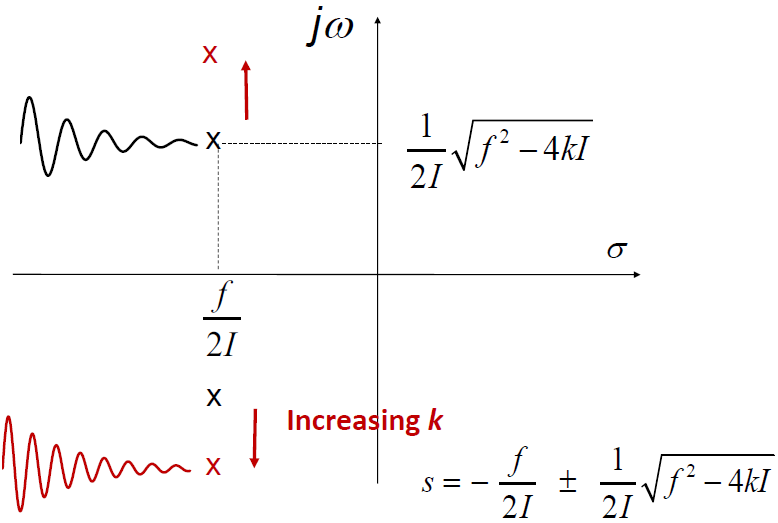
\includegraphics[width = 0.6\textwidth]{../img/diagram97.png}}
  \caption{}
\end{figure}
The behaviour is also apparent from the fact that the gain term $k$ affects both $\omega_n$ and $\zeta$ in an inversely related manner. The real part of the pole is given by $\omega_n \zeta$, so the increase in $\omega_n$ is cancelled out by decrease in $\zeta$.
\begin{equation}
  s = \zeta \omega_n \pm \omega_n \sqrt{\zeta^2 - 1}
\end{equation}
\subsubsection{Changing friction}
Changing the friction coefficient $f$ has a more complicated change on the pole location as it is located both in the real and imaginary components of the complex poles, and does not change $\omega_n$.
\begin{equation}
  s = - \frac{f}{2I} \pm \frac{1}{2I} \sqrt{f^2 - fkI}
\end{equation}
\begin{figure}[H]
  \centerline{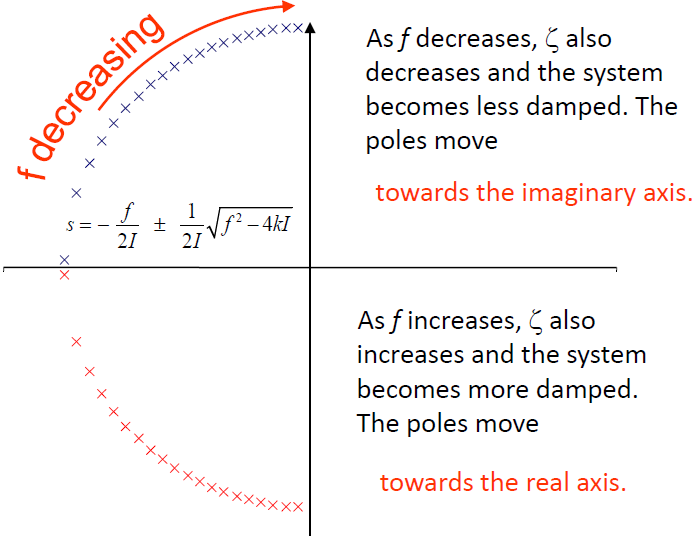
\includegraphics[width = 0.8\textwidth]{../img/diagram98.png}}
  \caption{}
\end{figure}
Most servos are designed with a low friction coefficient in mind, but this could increase with wear overtime for example, and thus the behaviour of the system would change.
\begin{figure}[H]
  \centerline{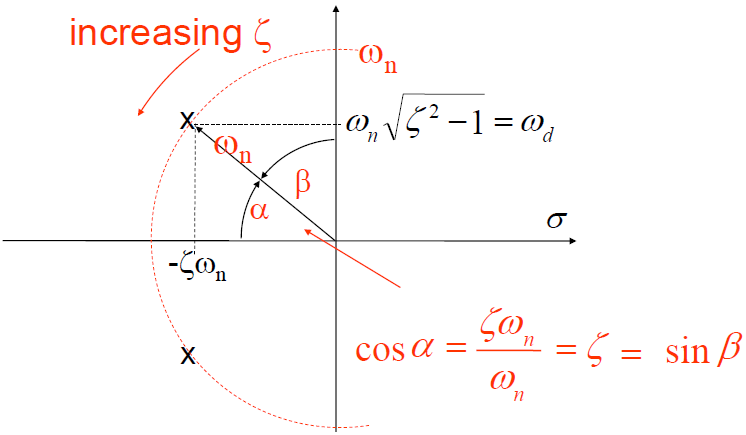
\includegraphics[width = 0.6\textwidth]{../img/diagram99.png}}
  \caption{}
\end{figure}
\subsubsection{Changing inertia}
Unlike the friction term, the inertia affects both the real and imaginary components of the complex poles. In this case, increasing the mass decreases the damping and the natural frequency. $\zeta = \frac{f}{2kI}$ (damping decreases), $\omega_n = \sqrt{\frac{k}{I}}$ (natural frequency decreases).
\begin{equation}
  s = - \frac{f}{2I} \pm \frac{1}{2I}\sqrt{f^2 - 4kI}
\end{equation}
\begin{figure}[H]
  \centerline{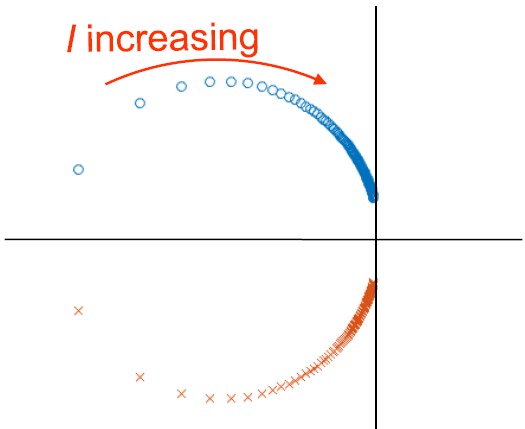
\includegraphics[width = 0.6\textwidth]{../img/diagram100.png}}
  \caption{}
\end{figure}
\section{Steady state performance}
Previously we have looked at performance criteria for the transient response of a system: settling time, peak time, overshoot etc. In addition to this, it is important to know hwo accurately the control system tracks the demand once it has settled down, i.e. it is in the steady state. For example in the ase of a ramp or step input:
\begin{figure}[H]
  \centerline{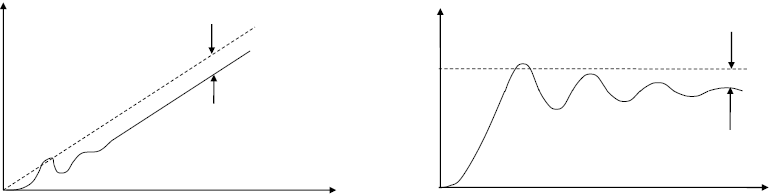
\includegraphics[width = 0.6\textwidth]{../img/diagram101.png}}
  \caption{}
\end{figure}
Steady state does not imply systems is not in motion! - e.g. can be moving at constant velocity, or oscillating.
\subsection{Final value theorem (FVT)}
For this we can use the final value theorem, which takes advantage of some handy properties of the Laplace transform. 
\begin{figure}[H]
  \centerline{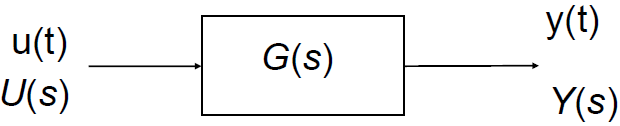
\includegraphics[width = 0.6\textwidth]{../img/diagram102.png}}
  \caption{}
\end{figure}
For a constant input, the output will (for some systems) settle down to a steady value that is a multiple of the input. The final value theorem gives the final value reached as:
\begin{align}
  \lim_{t\rightarrow \infty} y(t) = \lim_{s\rightarrow 0} s Y(s)
\end{align}
Note the extra $s$ term in $\lim_{s\rightarrow 0} s Y(s)$. So, the final value is found by setting $s$ to zero in the Laplace representation of the output and multiplying by $s$. There are two checks performed in control theory which confirm valid results for the Final Value Theorem:
\begin{enumerate}
  \item $Y(s)$ should have no poles in the right half the complex plane.
  \item $Y(s)$ should have no poles on the imaginary axis, except at most one pole at $s=0$.
\end{enumerate}
\begin{figure}[H]
  \centerline{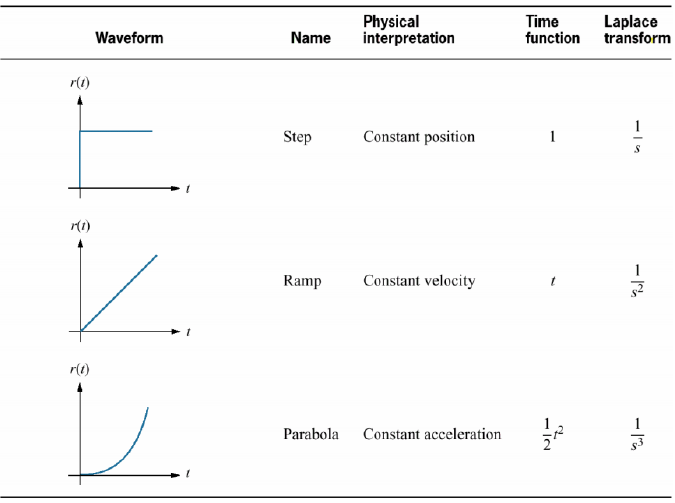
\includegraphics[width = 0.8\textwidth]{../img/diagram103.png}}
  \caption{}
\end{figure}
\subsection{Steady state error}
We are normally more interested in the final value of the error rather than the output, as the goal of the controller is to drive the error as close to zero. Further for some inputs such as ramp or sinusoidal input, the final output is not really meaningful.
\begin{figure}[H]
  \centerline{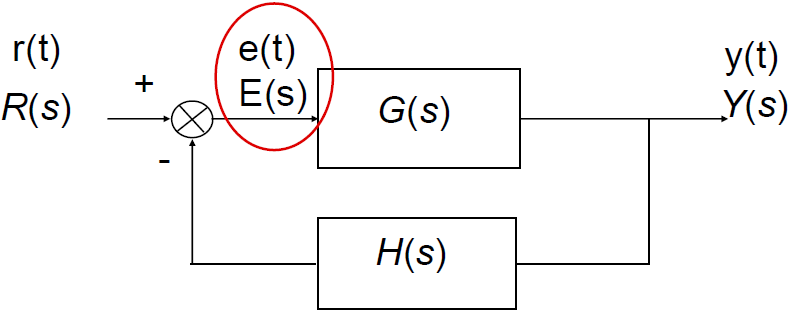
\includegraphics[width = 0.6\textwidth]{../img/diagram104.png}}
  \caption{}
\end{figure}
So, we first need to write the error signal with respect to the input:
\begin{align}
  E(s) &= R(s) - H(s)Y(S)\\
  Y(s) &= G(s)E(s)
\end{align}
So:
\begin{gather}
  E = R - HGE \rightarrow E + HGE = R\\
  E = \frac{R}{1+GH}
\end{gather}
Therefore, the final value of the error signal $e(t)$ would be:
\begin{align}
  \lim_{t\rightarrow \infty} e(t) = \lim{s\rightarrow 0} sE(s)
\end{align}
with
\begin{align}
  E(s) = \frac{R(s)}{1 + G(s) H(s)}
\end{align}
so
\begin{align}
  \lim_{s\rightarrow 0} s E(s) = \lim_{s\rightarrow 0} \frac{sR(s)}{1 + G(s) H(s)}
\end{align}
\subsection{Steady state position error}
Using the final value theorem, it is possible to find the steady state error of the control system and thus judge the appropriateness/success of the controller without having to calculate the full dynamic response at all. Remembering back to how long that took with only a second order system, you can imagine how useful this is!
\subsubsection{Step input demand}
\begin{align}
  R(s) &= \frac{A}{s}\\
  E(s) &= \frac{R(s)}{1 + G(s)H(s)}
\end{align}
Thus the final error is:
\begin{align}
  \lim_{t\rightarrow 0} e(t) &= \lim_{s\rightarrow 0} \frac{sR(s)}{1 G(s) H(s)} = \lim_{s\rightarrow 0} = \frac{s\frac{a}{s}}{1 + G(s)H(s)}
  &= \lim_{s\rightarrow 0} \frac{a}{1 +G(s)H(s)} = \frac{a}{1+k_p}
\end{align}
where $k_p = \lim_{s\rightarrow 0} G(s) H(s)$ is the position error constant.
\begin{figure}[H]
  \centerline{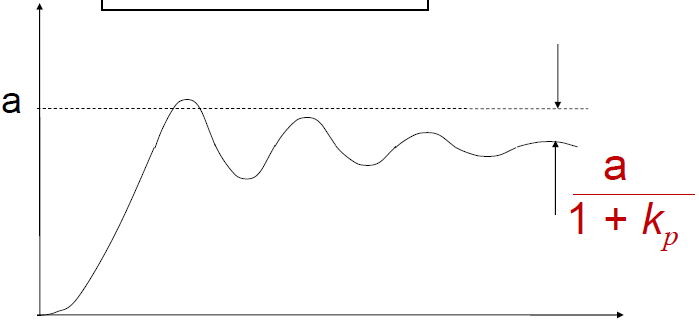
\includegraphics[width = 0.6\textwidth]{../img/diagram105.png}}
  \caption{}
\end{figure}
\subsection{Steady state velocity lag}
\subsubsection{Ramp input demand}
\begin{align}
  R(s) &= \frac{A}{s^2}\\
  E(s) &= \frac{R(s)}{1 + G(s)H(s)}
\end{align}
Thus the final error is:
\begin{align}
  \lim_{t\rightarrow \infty} e(t) &= \lim_{s\rightarrow 0} \frac{sR(s)}{1 + G(s)H(s)} = \lim_{s\rightarrow 0} \frac{s\frac{a}{s^2}}{1 + G(s)H(s)}\\
  &= \lim_{s\rightarrow 0} \frac{a}{s + sG(s) H(s)} = \frac{a}{k_v}
\end{align}
where $k_v = \lim_{s\rightarrow 0} sG(s) H(s)$ is the velocity error constant.
\begin{figure}[H]
  \centerline{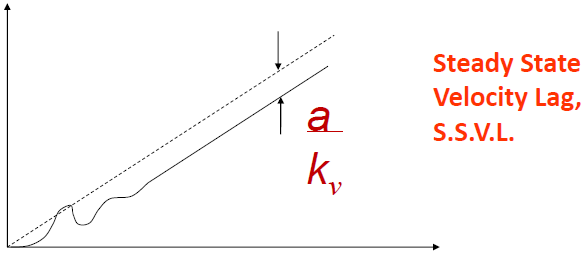
\includegraphics[width = 0.6\textwidth]{../img/diagram106.png}}
  \caption{}
\end{figure}
Once again, lets return to the servo example to see how this system would perform given these inputs.
\subsection{Servo steady state error}
\begin{figure}[H]
  \centerline{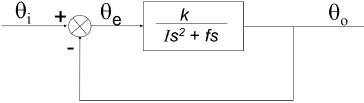
\includegraphics[width = 0.6\textwidth]{../img/diagram107.png}}
  \caption{}
\end{figure}
\subsubsection{Step input}
For a unity gain the steady state error is given by $\frac{a}{1 + k_p}$.
\begin{align}
  k_p &= \lim_{s\rightarrow 0} G(s)H(s)\\
  k_p &= \lim_{s\rightarrow 0} G(s) = \frac{k}{0\cdot (I\cdot 0 + f)} = \infty\\
  \lim_{t\rightarrow \infty} \theta_e (t) &= \frac{a}{1+k_p} = 0
\end{align}
So the position error is zero for all stable gains for a step input, i.e. the servo matches the demand completely.
\subsubsection{Ramp input}
Velocity error constant:
\begin{align}
  k_v = \lim_{s\rightarrow 0} sG(s) = \frac{k}{Is +f} = \frac{k}{f}
\end{align}
Steady state velocity error:
\begin{align}
  \lim_{t\rightarrow \infty} \theta (t) = \frac{a}{k_v} = \frac{af}{k}
\end{align}
This is the lag we saw in Lecture 5 when calculating the ramp response directly.
\end{document}